\section{P4}

%TODO redefine code listing package thingy

%TODO expand with exercise knowledge / what have we seen

For this summary, the focus is on P4$_{16}$ and the \href{https://p4.org/p4-spec/docs/P4-16-v1.2.1.html}{P4 language specification version 1.2.1}. All concepts seen here are taken from the lecture and exercises only - of course, there is much more to the language, refer to the documentation for more. The following is a list of very helpful resources to get to know the P4 programming language:

\begin{itemize}
    \item \href{https://p4.org/p4-spec/docs/P4-16-v1.2.1.html}{P4 language specification version 1.2.1}
    \item \href{https://github.com/p4lang/p4c/blob/master/p4include/v1model.p4}{P4-16 declaration of the v1.0 switch model}
    \item \href{https://github.com/nsg-ethz/p4-learning}{P4 learning repository}
    \item \href{https://gitlab.ethz.ch/nsg/public/adv-net-2020/-/tree/master/}{All exercises of the lecture (including some non-P4 stuff like FRR)}
\end{itemize}

%TODO more

\subsection{Basics}

%TODO example program

\paragraph{Program Structure}
A P4 program consists of imported libraries (by using the \texttt{\#include <name.p4>} command), constant / variable declarations, a parser, the control flow (match-action pipeline), a deparser and a call to main.

To maintain state between packets, use tables or externs (register, etc.).

The only loop possible in P4 is when we need to parse a header stack.

The most basic function of a switch (L2) is to compute the next hop, update the MAC addresses, decrease the TTL and forward it to the right egress port.

\paragraph{Base Types}
P4 is statically-typed and includes base types, as well as operators to derive composed ones (see below). Base types include (there is no float or string):

\begin{itemize}
    \item \texttt{bool}, default false
    \item \texttt{bit<n>}, width n, default 0
    \item \texttt{int<n>}, signed int, width n, default 0
    \item \texttt{varbit<n>}, dynamic length $\leq$ n
    \item etc.
\end{itemize}


\paragraph{Constant and Variable Declarations}
Declare constants and variables with these constructs (examples): 

\begin{itemize}
    \item \texttt{const bit<16> TYPE\_IPV4 = 0x800;}
    \item \texttt{typedef bit<32> ip4Addr\_t;}
    \item \texttt{header ip4\_t \{...\}}
    \item \texttt{struct headers \{...\}} or \texttt{struct metadata \{...\}} - unordered collection of named members
    \item \texttt{tuple<bit<32>, bool> x;} with \texttt{x = \{10, false\};} - unordered collection of unnamed members
\end{itemize}


%TODO tuples

\paragraph{Operations}
P4 includes arithmetic operations (add, sub, mult) without division and modulo, bitwise operators (complement, and, or, bit shift, xor), relation operators (smaller, bigger, equal, etc.), bit-slicing / concatenation, etc. 

\paragraph{Header Type}
The \texttt{header} type is similar to a \texttt{struct} in C and contains all the fields of the header to be defined at the beginning of the program. A header cannot be nested and contains a hidden Boolean validity field - the header is valid if this bit is true (use \texttt{isValid(), setValid(), setInvalid()} to manipulate it). A successful \texttt{extract()} during the parsing stage sets the validity bit to true. Example:

\begin{lstlisting}
header Ethernet_h {
   bit<48> dstAddr;
   bit<48> srcAddr;
   bit<16> etherType;
}
\end{lstlisting}

To declare a header, use \texttt{Ethernet\_h ethernetHeader;} or \texttt{MPLS\_h[10] mpls;} for a header stack with size 10. Headers are often combined by declaring them in a \texttt{struct} with the name \texttt{headers}. One can also define a \texttt{header\_union} where only one included alternative can be present (e.g. IPv4 vs. IPv6).

\paragraph{Metadata}
Intermediate data generated and / or manipulated during the execution of a P4 program and only associated with a single packet (if not used in combination of some kind of memory like registers). Can either be user-defined or is intrinsic to the underlying architecture model used (\texttt{struct standard\_metadata\_t}) - e.g. the ingress port of the packet or timestamps. %TODO: more? 

For this lecture, the architecture used is the \textit{v1model.p4}.

\paragraph{Externs}
Blackbox functions with a known interface and intrinsic to the architecture model used (kinda like Java interfaces). Can also be described as stateful objects. The \textit{v1model.p4} includes registers that store arbitrary data, counters, meters that can limit the rate, etc.

\begin{figure}[h]
	\centering
	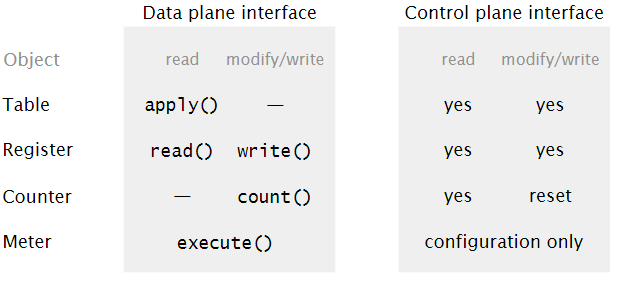
\includegraphics[scale=0.6]{images/6-externs.PNG}
	\caption{Stateful objects in P4 / v1model.}
	\label{fig:externs}
\end{figure}

%TODO: more on reg, counter, meter

\paragraph{Directional Parameters}
A function can take \texttt{in} parameters (only read inside the function), \texttt{out} parameters (uninitialized and written inside function, return values) and \texttt{inout} parameters (kinda like call-by-reference). Action parameters resulting from a table lookup (see below) don't have a direction since they come from the control plane.

\subsubsection{Parser}

%TODO what happens if reject - just dropped?
%TODO: in, out, inout things, function inputs

The parser maps packets into headers and metadata used and manipulated during the control flow stage of the P4 processing pipeline. It always needs to have a \texttt{start} state. In every state, one can transition into another state, which may depend on some condition, or transition into the \texttt{accept} resp. \texttt{reject} state (which is the default if no transition is specified). 

There are more advanced concepts that can be used in a parser (error handling with verify, accessing bits that are not parsed yet with lookahead, subroutines with sub-parser) - not really used during lecture / exercises. %TODO right?

Example of a common parser, with which we can later use \texttt{hdr}, \texttt{meta} and \texttt{standard\_metadata} of an IPv4 TCP resp. UDP packet:

\begin{lstlisting}
parser MyParser(packet_in packet,
                out headers hdr,
                inout metadata meta,
                inout standard_metadata_t standard_metadata) {

    state start{
        transition parse_ethernet;
    }
    
    state parse_ethernet{
        packet.extract(hdr.ethernet);
        transition select(hdr.ethernet.etherType){
            0x800: parse_ipv4;
            default: accept:
        }
    }
    
    state parse_ipv4{
        packet.extract(hdr.ipv4);
        transition select(hdr.ipv4.protocol){
            6: parse_tcp;
            17: parse_udp;
            default: accept;
        }
    }
    
    {...}
}

\end{lstlisting}


\subsubsection{Match-Action Pipeline}

After parsing the incoming packet, its checksum can be verified, ingress and egress processing is applied and its checksum can be updated - all using the information extracted during the parsing stage. All of these stages are divided into their own control blocks which are kinda like methods. Each block can contain its own variable and constant declarations and will most likely contain action and table declarations (= match-action units) and an (empty) apply statement defining the control flow.

\paragraph{Packet Checksum}
hmm, ip thingy %TODO

\paragraph{Ingress vs. Egress Processing}
I have no idea what the difference is. For the purpose of this lecture and the exercises, we almost always only defined any code in the ingress stage. %TODO

\paragraph{Processing Control}
An ingress / egress control block almost always contains constant / variable declarations, actions, tables and an apply statement. More advanced concepts include packet cloning, sending packets to the control plane and recirculating a packet.

\paragraph{Action}
Defines a function called when matching a specific key in a table. Can have zero or many input values extracted during the parsing stage.


\begin{lstlisting}
action drop() {
    mark_to_drop(standard_metadata);
}

action ipv4_forward(macAddr_t dstAddr, egressSpec_t port) {
    hdr.ethernet.srcAddr = hdr.ethernet.dstAddr;
    hdr.ethernet.dstAddr = dstAddr;
    standard_metadata.egress_spec = port;
    hdr.ipv4.ttl = hdr.ipv4.ttl - 1;
}
\end{lstlisting}

\paragraph{Table}
The control plane of a switch keeps track of all the tables used to process a passing packet. A table maps one or multiple given keys (header or metadata values extracted from the packet or else) to one of possibly many defined actions. The actual content of a table is filled by and stored in the control plane, while the structure of it is defined in the P4 program.

%TODO: how to fill

\begin{lstlisting}
table mpls_tbl {
    key = {
        hdr.mpls.label: exact;
    }
    actions = {
        mpls_forward;
        drop; // could also be NoAction
    }
    default_action = drop;
    size = CONST_MAX_LABELS;
}
\end{lstlisting}

\paragraph{Match Types}
A key can be matched either one-to-one (\texttt{exact}), longest prefix match (\texttt{lpm}) and ternary which TODO . The \textit{v1model.p4} also includes range match (check if a value is between x and y).

%TODO more detail, ternary

\paragraph{Filling a Table}
The .json topology object that describes all nodes and connections of a network also includes the possibility to define a .txt input file that defines CLI commands for a specific switch. To fill a table of a switch, the .txt file includes lines like:

\texttt{table\_add table\_name action\_name key $=>$ input\_1 ... input\_n}

\paragraph{Apply Statement}
Defines when to apply which table (and more). Can use if-else, switch, etc. statements. Example:

%TODO: more, switch example

\begin{lstlisting}
apply {
    table_1.apply();
    
    // Is it an IPv4 packet?
    if(hdr.ipv4.isValid()){
        table_2.apply();
    }
    
    // Apply table and check if there is a hit
    if(table_3.apply().hit){...}
    
    // Apply table and check which action is executed
    switch(table_4.apply().action_run){
        action1: {...}
        action2: {...}
    }
    
    {...}
}
\end{lstlisting}




\subsubsection{Deparser}
Puts packet back together s.t. it can be processed by regular switches in the network. Example: %order? if else stuff

\begin{lstlisting}
control MyDeparser(packet_out packet, in headers hdr) {
    apply {
        packet.emit(hdr.ethernet);
        packet.emit(hdr.mpls);
        packet.emit(hdr.ipv4);
    }
}
\end{lstlisting}